\documentclass[conference]{IEEEtran}

%XXX Remove before final submission
\usepackage{todonotes}
\usepackage{cite}
\usepackage{amsmath}
\usepackage{caption}
\usepackage{subcaption}
\usepackage{subcaption}
\usepackage[linesnumbered,ruled,vlined]{algorithm2e}
% Note that the amsmath package sets \interdisplaylinepenalty to 10000
% thus preventing page breaks from occurring within multiline equations. Use:
%\interdisplaylinepenalty=2500
% after loading amsmath to restore such page breaks as IEEEtran.cls normally
\usepackage{url}
\usepackage{hyperref}
\usepackage{verbatim}
\usepackage{siunitx}
\usepackage{listings}
\usepackage{mathtools}
\usepackage{float}

\DeclarePairedDelimiter\ceil{\lceil}{\rceil}
\DeclarePairedDelimiter\floor{\lfloor}{\rfloor}

\lstdefinelanguage{Julia}{
  basicstyle=\small\ttfamily,
  showspaces=false,
  showstringspaces=false,
  keywordstyle={\textbf},
  morekeywords={if,else,elseif,while,for,begin,end,quote,try,catch,return,local,abstract,function,stagedfunction,macro,ccall,finally,typealias,break,continue,type,global,module,using,import,export,const,let,bitstype,do,in,baremodule,importall,immutable},
  escapeinside={~}{~},
  morecomment=[l]{\#},
%  commentstyle=\textsf,
  commentstyle={},
  morestring=[b]",
}

\lstset{language=Julia,basicstyle=\footnotesize\ttfamily,breaklines=true}

% correct bad hyphenation here
\hyphenation{}


\begin{document}

%XXX remove before submission
\newcommand{\TODO}[1]{\todo[inline]{#1}}
\newcommand{\TODOFIG}[1]{\missingfigure{#1}}

\title{Catchy Title Here}

% author names and affiliations
% use a multiple column layout for up to three different
% affiliations
\author{\IEEEauthorblockN{Jiahao Chen and Jarrett Revels}
\IEEEauthorblockA{Computer Science and Artificial Intelligence Laboratory\\
Massachusetts Institute of Technology\\
Cambridge, Massachusetts 02139--4307\\
Email: \{jiahao,jrevels\}@csail.mit.edu}
}

% make the title area
\maketitle

\TODO{come up with better section/subsection names}
\TODO{come up with the final title}

%%%%%%%%%%%%%%%%%%%%%%%%%%%%%%%%%%%%%%%%%%%%%%%%%%%%%%%%%%%%%%%%%%%%%%%%%%%%%%%%%%%%%%%%%%%%
\begin{abstract}
We propose a robust methodology for automated benchmarking in the presence of timer error,
OS jitter and other environmental fluctuations. Motivated by data obtained from Julia
benchmarks, we demonstrate the ways in which timing distributions can violate assumptions
inherent to the statistical techniques employed by other benchmarking frameworks. From our
experimental observations, we construct a model and an accompanying strategy for estimating
program execution time which purposefully avoids these assumptions. This strategy makes
efficient use of experimental time constraints by simultaneously maximizing the number of
measurements per trial while minimizing inter-measurement timing variations, rendering it
suitable for continuous integration (CI) pipelines, even when applied to relatively large
benchmark suites. Additionally, we discuss the advantages and disadvantages of different
approaches to hypothesis testing in a non-i.i.d. setting, arguing in favor of further
investigation of block resampling methods for future work on statistical performance
regression detection. Finally, we describe the implementation of the benchmarks used to
perform our experiments. These benchmarks are written using the BenchmarkTools package, a
Julia implementation of this paper's methodology that is currently used in the development
of the Julia language and ecosystem.
\end{abstract}

\IEEEpeerreviewmaketitle

%%%%%%%%%%%%%%%%%%%%%%%%%%%%%%%%%%%%%%%%%%%%%%%%%%%%%%%%%%%%%%%%%%%%%%%%%%%%%%%%%%%%%%%%%%%%
\section{Introduction}
\label{sec:intro}

Developers of high performance applications often rely on benchmark suites to determine the
impact of code changes on program performance. Despite the importance of these suites in
safeguarding against performance regressions, developers often execute and interpret them in
an ad hoc manner. This disregard for proper experimental methodology wastes development time
and may lead to misguided decisions that worsen performance.

In this paper, we consider the problem of designing a language- and platform-agnostic
benchmarking methodology that is suitable for continuous integration (CI) pipelines and
manual user workflows. Our methodology especially focuses on the accommodation of benchmarks
whose expected executions times are short enough that timing measurements are vulnerable to
error due to insufficient system timer accuracy (generally on the order of microseconds
or less).

\subsection{Accounting for performance variations}
\label{sec:variations}

Modern hardware and operating systems introduce many confounding factors that complicate a
developer's ability to reason about variations in user-space application
performance~\cite{HP5e}. Timing measurements can exhibit correlation structures that depend
on a myriad of factors such as environment temperature, workload, power availability, and
network traffic, and operating system (OS) configuration. For the sake of stabilize and
improve program performance, a significant portion of performance testing research is
focused on identifying and isolating (or eliminating) sources of variation.

Over the past decade and a half, system quiescence research has uncovered a large number of
these sources stemming from OS behaviors, including CPU frequency scaling \cite{RHEL6},
address space layout randomization (ASLR)~\cite{Shacham2004}, virtual memory
management~\cite{Oyama2014,Oyama2016}, differences between CPU privilege
levels~\cite{Zaparanuks2009}, context switches due to interrupt handling~\cite{Tsafrir2007},
activity from system daemons and cluster managers~\cite{Petrini2003}, and suboptimal
process- and thread-level scheduling~\cite{Lozi2016}. Even seemingly irrelevant
configuration parameters like the size of the OS environment can confound experimental
reproducibility by altering the alignment of data in memory~\cite{Mytkowicz2009}.

System quiescence research has also identified language-specific sources of performance
variation. For example, some languages feature linkers which are free to choose the binary
layout of the library or executable arbitrarily, resulting in non-deterministic memory
layouts~\cite{Georges2008}. This problem is exacerbated in languages like C++, whose
compilers introduce random name mangling of symbols~\cite{Kalibera2005}. Another class of
performance variations are due to unexpected compiler optimizations, which adversely affect
the accuracy of hardware counters~\cite{Zaparanuks2009}, or in extreme cases eliminate key
parts of the benchmark as dead code. Yet another example is garbage collector performance,
which can exhibit varying behavior based on external parameters such as heap
size~\cite{Blackburn2004}.

\subsection{Doing statistics on timing measurements is hard}
\label{sec:toughstats}

\begin{figure}
\centering
\begin{subfigure}{0.22\textwidth}
    \centering
    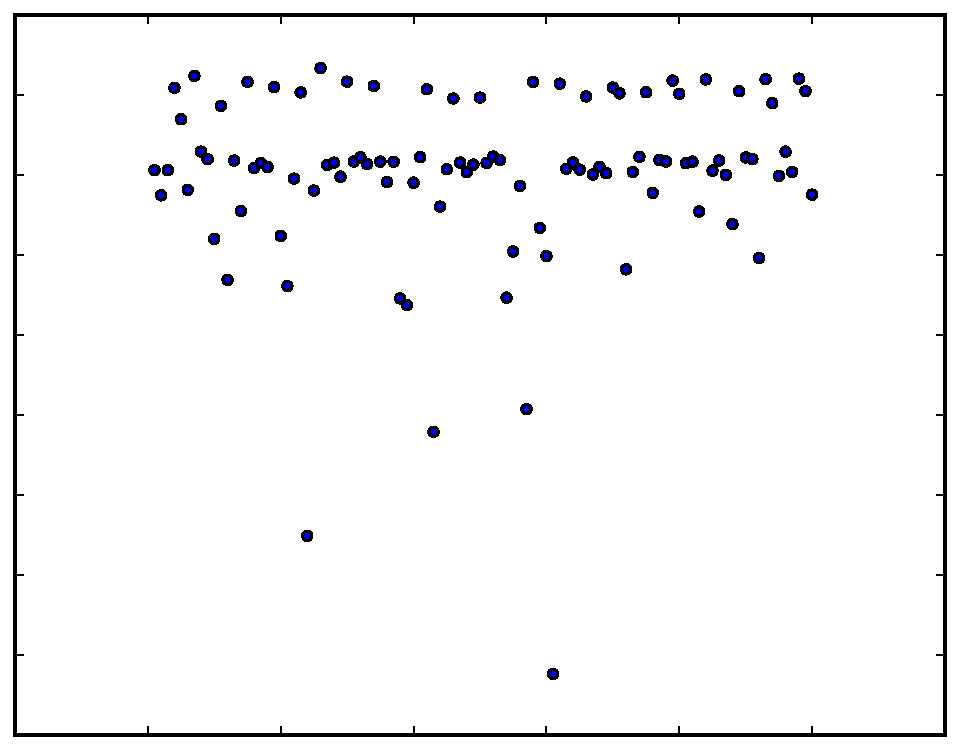
\includegraphics[width=\textwidth]{figures/fig1/simple_branchsum_fast}
    \caption{Benchmark 1: Unimodal with skew and large outliers}
\end{subfigure}%
~
\begin{subfigure}{0.22\textwidth}
    \centering
    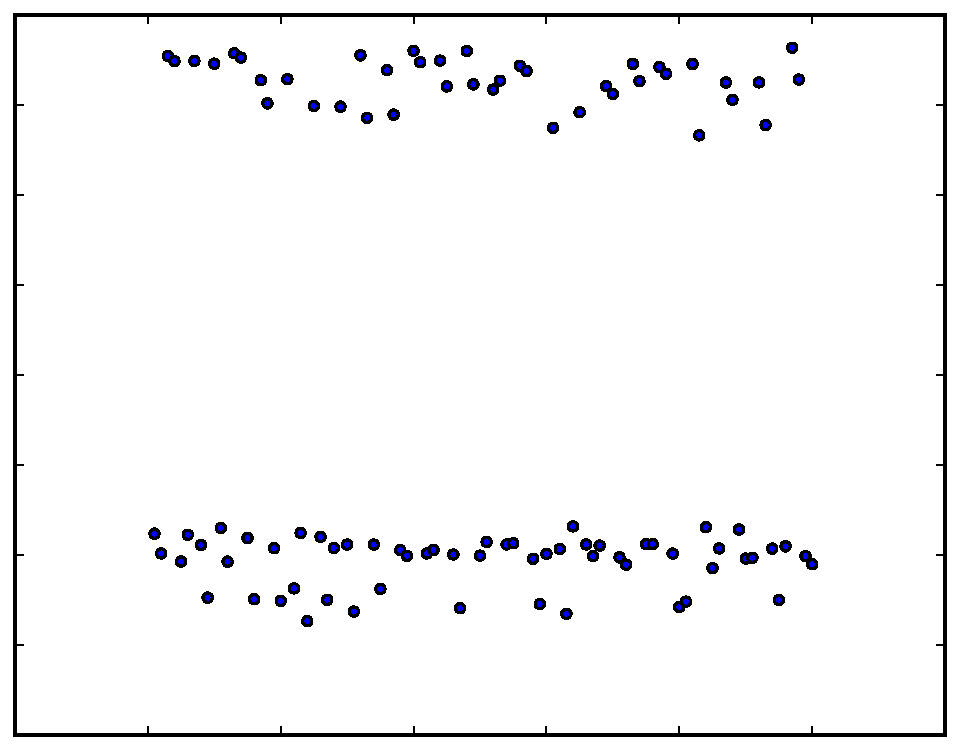
\includegraphics[width=\textwidth]{figures/fig1/bimodal_branchsum}
    \caption{Benchmark 2: Bimodal}
\end{subfigure}
\begin{subfigure}{0.22\textwidth}
    \centering
    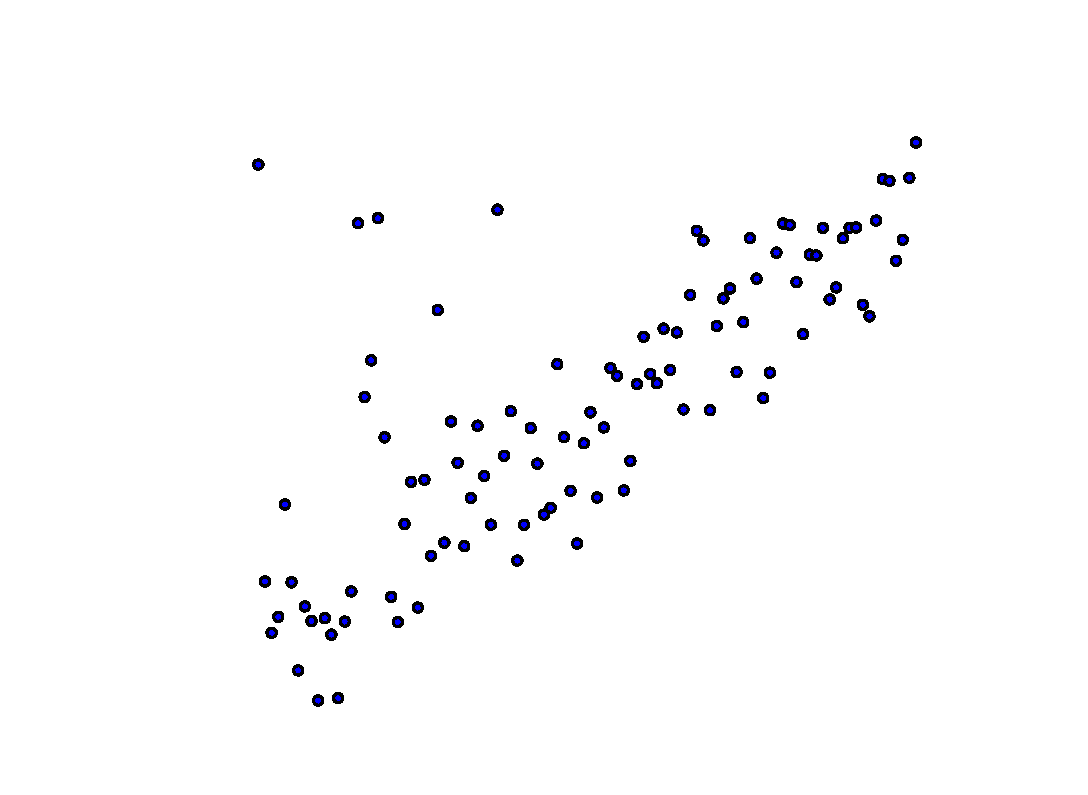
\includegraphics[width=\textwidth]{figures/fig1/drift_manyallocs_slow}
    \caption{Benchmark 3: Drift}
\end{subfigure}
~
\begin{subfigure}{0.22\textwidth}
    \centering
    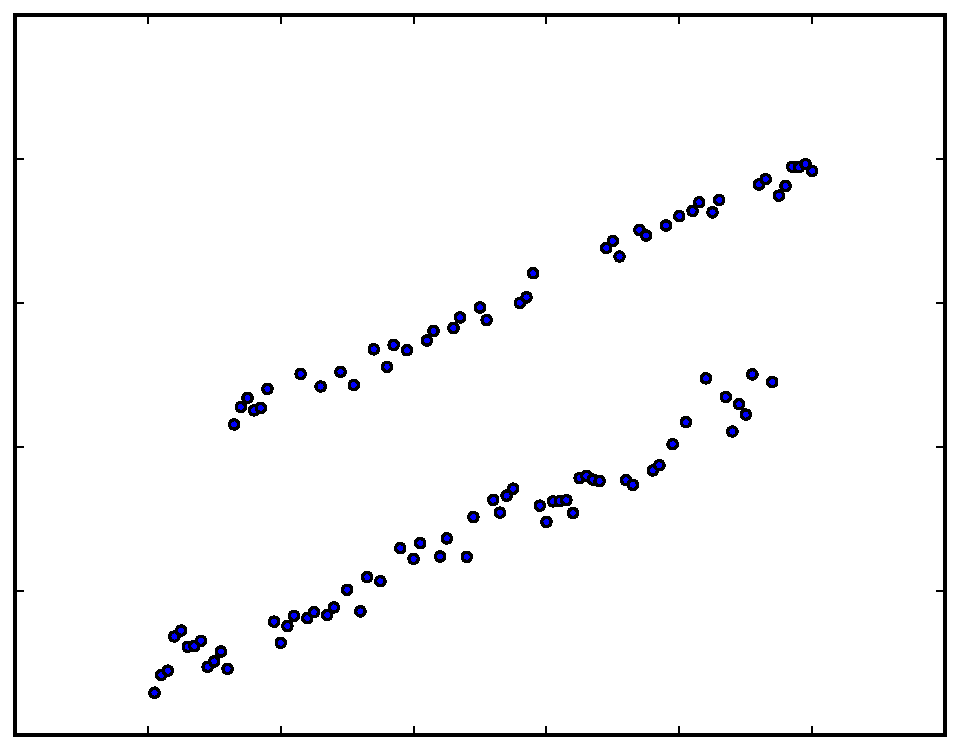
\includegraphics[width=\textwidth]{figures/fig1/bimodal_drift_sumindex}
    \caption{Benchmark 4: Bimodal with drift}
\end{subfigure}
\caption{Variability in the mean benchmark time across multiple trials, showing
that the mean has non-i.i.d., non-normal behavior in four different benchmarks.
Each point represents a mean time computed from trial of 10,000 measurements.
The horizontal axis is the index of the trial, while the vertical axis is time.}
\label{fig:meandistributions}
\vspace{-0.42cm} % hack to get rid of weirdly large line gap below this figure
\end{figure}

The myriad sources of performance variation discussed in the previous section pose a
significant problem when applying textbook statistical approaches to benchmark timing
measurements. Central to this problem is the violation of a commonly relied-upon assumption
that the sample mean will converge to a normal distribution as the sample size increases,
as would be the case if timing samples were independent and identically distributed (i.i.d.).

In reality, we have observed non-i.i.d. behavior in many Julia benchmarks. For example,
Figure~\ref{fig:meandistributions} shows that none of the four illustrative benchmarks
considered in this paper exhibit normality in the sample mean. Instead, we see that the mean
demonstrates skewed density and outliers in the first benchmark, bimodality in the second
and fourth benchmarks, and upward drift in the third and fourth benchmarks. This non-ideal
behavior has also been observed in other studies~\cite{Gil2011, Chen2015,
Rehn2015,Barrett2016}. In these situations, standard techniques such as $F$-tests or
Student's t-tests have poor statistical
power~\cite{Lilja2000,Mytkowicz2009,Kalibera2013,Chen2015, Barrett2016}. This problem can
also affect benchmarking software that tries to correct for non-ideal behavior by using
parametric outlier removal techniques, such as AndroBench's use of the 3-sigma rule
\cite{Kim2012}.

To combat non-ideal statistics, some authors propose methods for reducing external
performance variations, removing outliers, and artificially inducing normality in benchmark
programs. Such methods include custom OS kernels \cite{Tessellation,Akkan2012}, custom
compilers providing reproducible~\cite{Georges2008} or consistently
randomized~\cite{Curtsinger2013} binary layouts, to low-variability garbage
collectors~\cite{Huang2004}. Unfortunately, the implementation and applicability of these
methods are often specific to a single programming language, compiler, and/or platform.
Furthermore, these methods often require drastic modifications to a typical user's
workspace, which cannot be reasonably automated without root access to a user's machine.

\subsection{Existing benchmarking methodologies}
\label{sec:existingtools}

While it is impossible to eliminate performance variation
entirely~\cite{Alcocer2015,Barrett2016}, benchmarking methodologies that attempt to account
for both measurement error and external sources of variation do exist.

For example, the Haskell microbenchmarking packages \lstinline|criterion|~\cite{criterion}
attempts to thwart error due to timer inaccuracy by growing the number of benchmark
executions per timing measurement as more timing measurements are obtained. After all
measurements are taken, a summary estimate of the benchmark runtime is obtained by examining
the derivative of the ordinary least squares regression line at the point of a single
evaluation point. The disadvantages of this strategy are threefold. First, the least squares
fit employed by \lstinline|criterion| is sensitive to outliers (though \lstinline|criterion|
does print a warning to the user if outliers are detected)~\cite{Maronna2006}. Second,
measurements made earlier in this experiment are highly vulnerable to timer error, since few
benchmark repetitions are used. These early measurements can skew the regressions line, and
in turn, skew the final runtime estimate. Third, measurements made later in the experiment
can repeat the benchmark more times than is necessary to overcome timer error, constituting
an inefficient use of experimenter time.

One of the more promising methodologies is presented by Kalibera et al. in the paper
``Rigorous Benchmarking in Reasonable Time''~\cite{Kalibera2013}. Their approach is largely
platform-agnostic, recognizes the pitfalls of inter-measurement correlations, and
acknowledges that merely increasing the number of benchmark repetitions is not always a
sufficient strategy to yield i.i.d. samples. However, the downside of Kalibera et al.'s
methodology is that it requires the upfront execution of a manual experiment for every
benchmark, compiler, and platform combination. The initial cost of a manual experiment is a
low barrier to overcome if one is simply seeking benchmark results for research purposes,
but can render the methodology inaccessible for normal user workflows and CI pipelines,
where benchmark suites are large and change often. For example, the Julia language's
standard library benchmark suite contains over 1300 benchmarks, and is frequently expanded
to improve performance test coverage. For cases like these, it is vital that even
pre-experiment parameter tuning be automatable.

%%%%%%%%%%%%%%%%%%%%%%%%%%%%%%%%%%%%%%%%%%%%%%%%%%%%%%%%%%%%%%%%%%%%%%%%%%%%%%%%%%%%%%%%%%%%
\section{Notation}
\label{sec:notation}

The rest of this paper utilizes a consistent notation for discussing various statistical and
measured quantities related to benchmarking. We define this notation here:

\begin{itemize}
    \item
    $P_0$, $P$ and $Q$ denote \textbf{benchmarkable programs}, each defined by a tape of
    instructions.

    \item
    $I^{[i]}_{P}$ is the $i^{\textrm{th}}$ \textbf{instruction} in the tape defining program $P$.
    Instruction indices are always written using bracketed superscripts, $\cdot^{[i]}$.

    \item
    $D^{[i]}_{P}$ is the \textbf{delay instruction} associated with $I^{[i]}_{P}$. Delay
    instructions are precisely defined in Section~\ref{sec:model}.

    \item
    $T_i$ is a \textbf{timing measurement}. Specifically, $T_i$ is the amount of time taken
    to perform $n_i$ \textbf{executions} of a benchmarkable program. This quantity is
    directly measurable via experiment.

    \item
    $t$ is a \textbf{theoretical execution time}. $t_{P_0}$ is the minimum time required to
    perform a single execution of $P_0$ on a given computer.

    \item
    \textbf{Estimated quantities} are denoted with a hat, $\hat\cdot$. For example,
    $\hat{t}_{P_0}$ is an estimate of the theoretical execution time $t_{P_0}$.

    \item
    A benchmark \textbf{experiment} is a recipe for obtaining multiple timing measurements
    for a benchmarkable program. Experiments can be executed to obtain \textbf{trials}. The
    $i^{\textrm{th}}$ trial of an experiment is a collection of timing measurements
    $T^{\{i\}}_1, \dots T^{\{i\}}_j, \dots T^{\{i\}}_k$. Trial indices are always
    written using embraced superscripts, $\cdot^{\{i\}}$.

    \item
    $\tau$ denotes time quantities that are external to the benchmarkable program:
    \begin{itemize}
        \item $\tau_{\textrm{budget}}$ is the \textbf{time budget} for an experiment.
        \item $\tau_{\textrm{acc}}$ is the \textbf{accuracy} of the system timer.
        \item $\tau_{\textrm{prec}}$ is the \textbf{precision} of the system timer.
    \end{itemize}

    \item
    $x_P^{(i)[j]} \tau^{(i)}$ is the \textbf{time delay} due to the
    $i^{\textrm{th}}$ \textbf{delay factor} for delay instruction $D^{[j]}$.  Specifically,
    $\tau^{(i)}$ is the factor's \textbf{time scale} and $x_P^{(i)[j]}$ is the factor's
    \textbf{trigger coefficient}. Delay factor indices are written using parenthesized
    superscripts, $\cdot^{(i)}$.

    \item
    $\epsilon$ is the measurement error due to timer inaccuracy.

    \item
    $E_m$ is $\frac{T_m}{n_m} - t_{P_0}$ for a measurement $m$. In other words, $E_m$ is the
    \textbf{total contribution of all delay factors found in measurement $m$, plus the
    measurement error $\epsilon$}.

    \item
    $X^{(i)}_P$ is the \textbf{total trigger count} of the $i^{\textrm{th}}$
    delay factor during the execution of program $P$.

    \item
    $\nu$ is an \textbf{oracle function} that, evaluated at an execution time $t$, estimates
    an appropriate $n$ necessary to overcome measurement error due to insufficient
    $\tau_{\textrm{acc}}$ and $\tau_{\textrm{prec}}$.
\end{itemize}

%%%%%%%%%%%%%%%%%%%%%%%%%%%%%%%%%%%%%%%%%%%%%%%%%%%%%%%%%%%%%%%%%%%%%%%%%%%%%%%%%%%%%%%%%%%%
\section{A model for benchmark timing distributions}
\label{sec:model}

In this section, we present a statistical description of benchmark behavior that avoids
problematic assumptions of normality or identical timing distributions between benchmarks.
This model will drive the design of the experimental protocol and the hypothesis test
that we discuss in future sections.

\subsection{The definition and execution of benchmark programs}
\label{sec:programmodel}

Consider an initial benchmarkable user program $P_0$, whose output is deterministic and
identical for every execution of the program. For any given computer, $P_0$ can be
represented by some sequence of instructions $I^{[i]}$:

\begin{equation}
    P_0 = \left[I^{[1]}, I^{[2]}, \dots I^{[k]}\right]
\end{equation}

We denote the runtime of instruction $I^{[i]}$ as $\tau^{[i]}$, such that the total runtime
of $P_0$ can be written $t_{P_0} = \sum_{i=1}^N \tau^{[i]}$. Regardless of the code supplied
by $P_0$'s original author, the computer on which $P_0$ runs is free to execute any series
of instructions which implements the exact behavior of $P_0$ with respect to the scope of
$P_0$'s original definition and execution. For the purposes of our model, we will define
$\left[I^{[1]}, I^{[2]}, \dots I^{[k]}\right]$ to be a series of instructions which, if
executed by the computer exactly, minimizes $t_{P_0}$ across all possible configurations of
$\tau^{[i]}$.

In reality, the machine and operating system executing $P_0$ are vulnerable to the factors
described in Section~\ref{sec:variations}. Since these factors can \textit{delay} the
completion of the original instructions, we refer to them as \textit{delay
factors.}\footnote{Technically, there are some external factors which might speed up program
execution, such as frequency scaling~\cite{RHEL6}. However, these factors number far fewer
than those that slow down program execution. Thus, we only focus on the latter, which we
believe dominates the former in most real-world settings.} We can incorporate these delay
factors into our original program definition by modeling them as \textit{delay instructions}
$D^{[i]}$, which are interleaved with $P_0$'s original instructions to produce a new program
$P$:

\begin{equation}
    P = \left[I^{[1]}, D^{[1]}, I^{[2]}, D^{[2]}, \dots I^{[k]}, D^{[k]}\right]
\end{equation}

We assume that the delay instructions do not interfere with the semantics of $P_0$, such
that $P$ and $P_0$ share an identical mapping of inputs to outputs. Incorporating the delay
instructions, the runtime of $P$ can be written as

\begin{equation}
    t_P = t_{P_0} + \sum_{j} \tau^{[j]}_D
\end{equation}

where $\tau^{[j]}_D$ is the execution time of $D^{[j]}$. Since $\tau^{[j]}_D \ge 0$, it
follows that $t_P \ge t_{P_0}$.

$\tau^{[j]}_D$ can be further decomposed into the runtime contributions of individual delay
factors. Let us imagine the delay factor $i$ can discretely ``trigger'' once during the
execution of $D^{[j]}$ with probability $p^{(i)[j]}$. Assuming that every triggering of $i$
takes a fixed time $\tau^{(i)}$, then

\begin{equation}
    \tau^{[j]}_D = \sum_{i} x_P^{(i)[j]} \tau^{(i)}
\end{equation}

where $x_P^{(i)[j]}$ is a \textit{Bernoulli random variable} with success probability
$p^{(i)[j]}$. We denote the total number of times the $i^{\textrm{th}}$ delay factor was
triggered during the execution of $P$ as the \textit{trigger count} $X_P^{(i)} = \sum_{j}
x_P^{(i)[j]}$. Since the trigger count is a sum of independent Bernoulli random variables with
nonidentical success probabilities, $X_P^{(i)}$ is itself a random variable that follows a
\textit{Poisson binomial distribution} parameterized by the success probabilities
$\left[p^{(i)[1]}, \dots p^{(i)[k]}\right]$.

Our final expression for $t_P$ in terms of these quantities is:

\begin{align}
t_P &= t_{P_0} + \sum_{j} \tau^{[j]}_D \\ \nonumber
    &= t_{P_0} + \sum_{i} \sum_{j=1}^{k} x_P^{(i)[j]} \tau^{(i)} \\ \nonumber
    &= t_{P_0} + \sum_{i} X_P^{(i)} \tau^{(i)}
\end{align}

In summary, our model treats $t_P$ as a random variable whose distribution depends on the
trigger probabilities $p^{(i)[j]}$, which are determined by the combined behavior of the
delay factors and the initial benchmark program $P_0$.

\subsection{The effects of repeated benchmark execution}
\label{sec:measuremodel}

As mentioned in Section~\ref{sec:existingtools}, experiments which measure program
performance often incorporate multiple benchmark executions in an attempt to obtain more
accurate measurements. We will now apply our model to demonstrate that this strategy is
sufficient for eliminating timer error, but is not sufficient to obviate the effects of
delay factors.

To simplify our analysis, we can represent $n$ executions of a program $P_0$ comprised of
$k$ instructions as a single execution of a program $Q_0$, which is the result of
concatenating $n$ copies of $P_0$:

\vspace{-0.35cm}
\begin{align}
P_0 &= \left[I^{[1]}, I^{[2]}, \dots I^{[k]} \right] \\ \nonumber
Q_0 &= \left[P_0, P_0, \dots P_0 \right] \\ \nonumber
    &= \left[I_{P}^{[1]}, \dots I_{P}^{[k]}, I_{P}^{[1]}, \dots I_{P}^{[k]}, I_{P}^{[1]}, \dots I_{P}^{[k]} \right] \\ \nonumber
    &= \left[I_{Q}^{[1]}, I_{Q}^{[2]}, \dots I_{Q}^{[nk]} \right]
\end{align}

such that instruction $I_{P}^{[i]} = I_{Q}^{[i + ck]}$ for $c \in \{0, \dots n - 1\}$.
Following the convention of the previous section, we use $Q$ to denote the program that
results from interleaving $Q_0$ with delay instructions. Note that $Q$ is \textit{not}
simply $n$ repetitions of $P$, since $Q$'s delay instructions do not obey the repetition
relation of the original instructions ($D_{P}^{[i]} \ne D_{Q}^{[i + ck]}$).

An observed timing measurement $T$ of a single execution of $Q$ can be decomposed as
follows:

\vspace{-0.35cm}
\begin{align}
    T &= t_{Q} + \epsilon \\ \nonumber
      &= t_{Q_0} + \sum_{i} X_Q^{(i)} \tau^{(i)} + \epsilon \\ \nonumber
      &= n \cdot t_{P_0} + \sum_{i} \sum_{j=1}^{nk} x_Q^{(i)[j]} \tau^{(i)} + \epsilon
\end{align}

where $\epsilon$ is the error due to timer inaccuracy, subject to the
constraint $-\tau_{\textrm{acc}} \le \epsilon \le \tau_{\textrm{acc}}$.

We can obtain a naive estimate for $t_{P_0}$ by dividing $T$ by $n$:

\vspace{-0.10cm}
\begin{equation}
    \frac{T}{n} = t_{P_0} + \frac{\sum_{i} \sum_{j=1}^{nk} x_Q^{(i)[j]} \tau^{(i)} + \epsilon}{n}
\end{equation}

In the limit of large $n$, $\frac{\epsilon}{n}$ goes to zero, but the behavior of the delay
factor term is less clear:

\vspace{-0.10cm}
\begin{equation}  \label{eq:9}
    \lim_{n\to\infty} \frac{T}{n} = t_{P_0} + \lim_{n\to\infty} \frac{\sum_{i} \sum_{j=1}^{nk} x_Q^{(i)[j]} \tau^{(i)}}{n}
\end{equation}

While the exact behavior of the delay factor term depends on the random variables
$X_Q^{(i)}$, we can derive an achievable tight upper bound on the delay factor term whose
limit as $n \to \infty$ can be evaluated. Consider the worst case where all $x_Q^{(i)[j]} =
1$, such that all $X_Q^{(i)} = nk$. The delay factor term then reduces as:

\vspace{-0.35cm}
\begin{align} \label{eq:10}
    \sum_{i} \sum_{j=1}^{nk} x_Q^{(i)[j]} \tau^{(i)} &= \sum_{i} \sum_{j=1}^{nk} \tau^{(i)} \\ \nonumber
                                                     &= nk \sum_{i} \tau^{(i)}
\end{align}

Plugging Eq~\ref{eq:10} into Eq~\ref{eq:9}, we see that in the worst case the delay factor
term can dwarf $t_{P_0}$ regardless of the number of executions of $P_0$ performed during
the measurement:

\vspace{-0.35cm}
\begin{align} \label{eq:11}
    \lim_{n\to\infty} \frac{T}{n} &= t_{P_0} + \lim_{n\to\infty} \frac{nk \sum_{i} \tau^{(i)}}{n} \\ \nonumber
                                  &= t_{P_0} + k \sum_{i} \tau^{(i)}
\end{align}

Eq~\ref{eq:11} is a key result of our model: \textbf{One cannot reliably eliminate the
effects of external variations simply by executing the benchmark a large number of times.}
Whether or not increasing $n$ can render the delay factor term negligible depends entirely on
the random variables $X_Q^{(i)}$, which, recalling our discussion in
Section~\ref{sec:variations}, are not easily controlled in practice.

%%%%%%%%%%%%%%%%%%%%%%%%%%%%%%%%%%%%%%%%%%%%%%%%%%%%%%%%%%%%%%%%%%%%%%%%%%%%%%%%%%%%%%%%%%%%
\section{An Automated procedure for configuring performance experiments}
\label{sec:confexperiment}

In Section~\ref{sec:measuremodel}, we found that increasing $n$, the number of benchmark
executions per timing measurement, is not a sufficient strategy to eliminate the effects of
delay factors on timing measurements. However, we showed that increasing $n$ can improve
timing measurements by eliminating error due to timer inaccuracy. In this section, we
present an experimental procedure for automatically selecting useful values of $n$ for
a given benchmark program.

\subsection{An algorithm for estimating the optimal $n$ value}

Given $P_0$ (the initial benchmarkable program), $n$ (the number of executions of $P_0$ per
timing measurement), and $\tau_{\textrm{budget}}$ (the user's time budget), an experiment
consists of making several timing measurements $T_1, \dots T_m$ until we have exhausted
$\tau_{\textrm{budget}}$.

Since $P_0$ and $\tau_{\textrm{budget}}$ are fixed by the user, the only parameter we are
free to optimize is $n$. Recalling our model, increasing $n$ can cause $\frac{\epsilon}{n}
\to 0$, thus increasing the accuracy of our estimates $\frac{T_1}{n}, \dots \frac{T_m}{n}$.
However, increasing $n$ also increases the time required to perform a single measurement,
thus decreasing $m$, the number of measurements we can take within the time budget. We can
strike a reasonable balance between maximizing measurement accuracy and maximizing $m$ by
guessing a minimal value of $n$ that renders $\frac{\epsilon}{n} \ll t_{P_0}$. Our
automatable procedure for guessing this value is given in Algorithm~\ref{alg:tuning}:

\begin{algorithm}
    \caption{estimating the optimal $n$ value}
    \label{alg:tuning}
    \KwIn{$P_0$, $\tau_{\textrm{acc}}$, $\tau_{\textrm{prec}}$, an oracle function $\nu : t \to n$}
    \KwOut{$n$}
    Let $j = \tau_{\textrm{acc}} / \tau_{\textrm{prec}}$.

    For $i \in \{1, \dots j\}$, measure the amount of time it takes to perform $i$
    executions of $P_0$, resulting in a collection of timing measurements $T_1, \dots T_j$.

    Estimate $t_{P_0}$ as $\hat{t}_{P_0} = \textrm{min}(\frac{T_1}{1}, \dots \frac{T_j}{j})$.

    Evaluate $\nu(\hat{t}_{P_0})$ to obtain $n$.
\end{algorithm}

An extensive description of the oracle function and its purpose is provided in
Section~\ref{sec:oracle}.

Note that Algorithm~\ref{alg:tuning} only ever needs to be applied once per benchmark, since
the estimated $n$ can be cached for use in subsequent experiments. Thus, we consider this
algorithm an automated pre-processing step that does not count against our time budget
$\tau_{\textrm{budget}}$.

\subsection{Justifying the minimum estimator}
\label{sec:minimum}

\begin{figure}
\centering
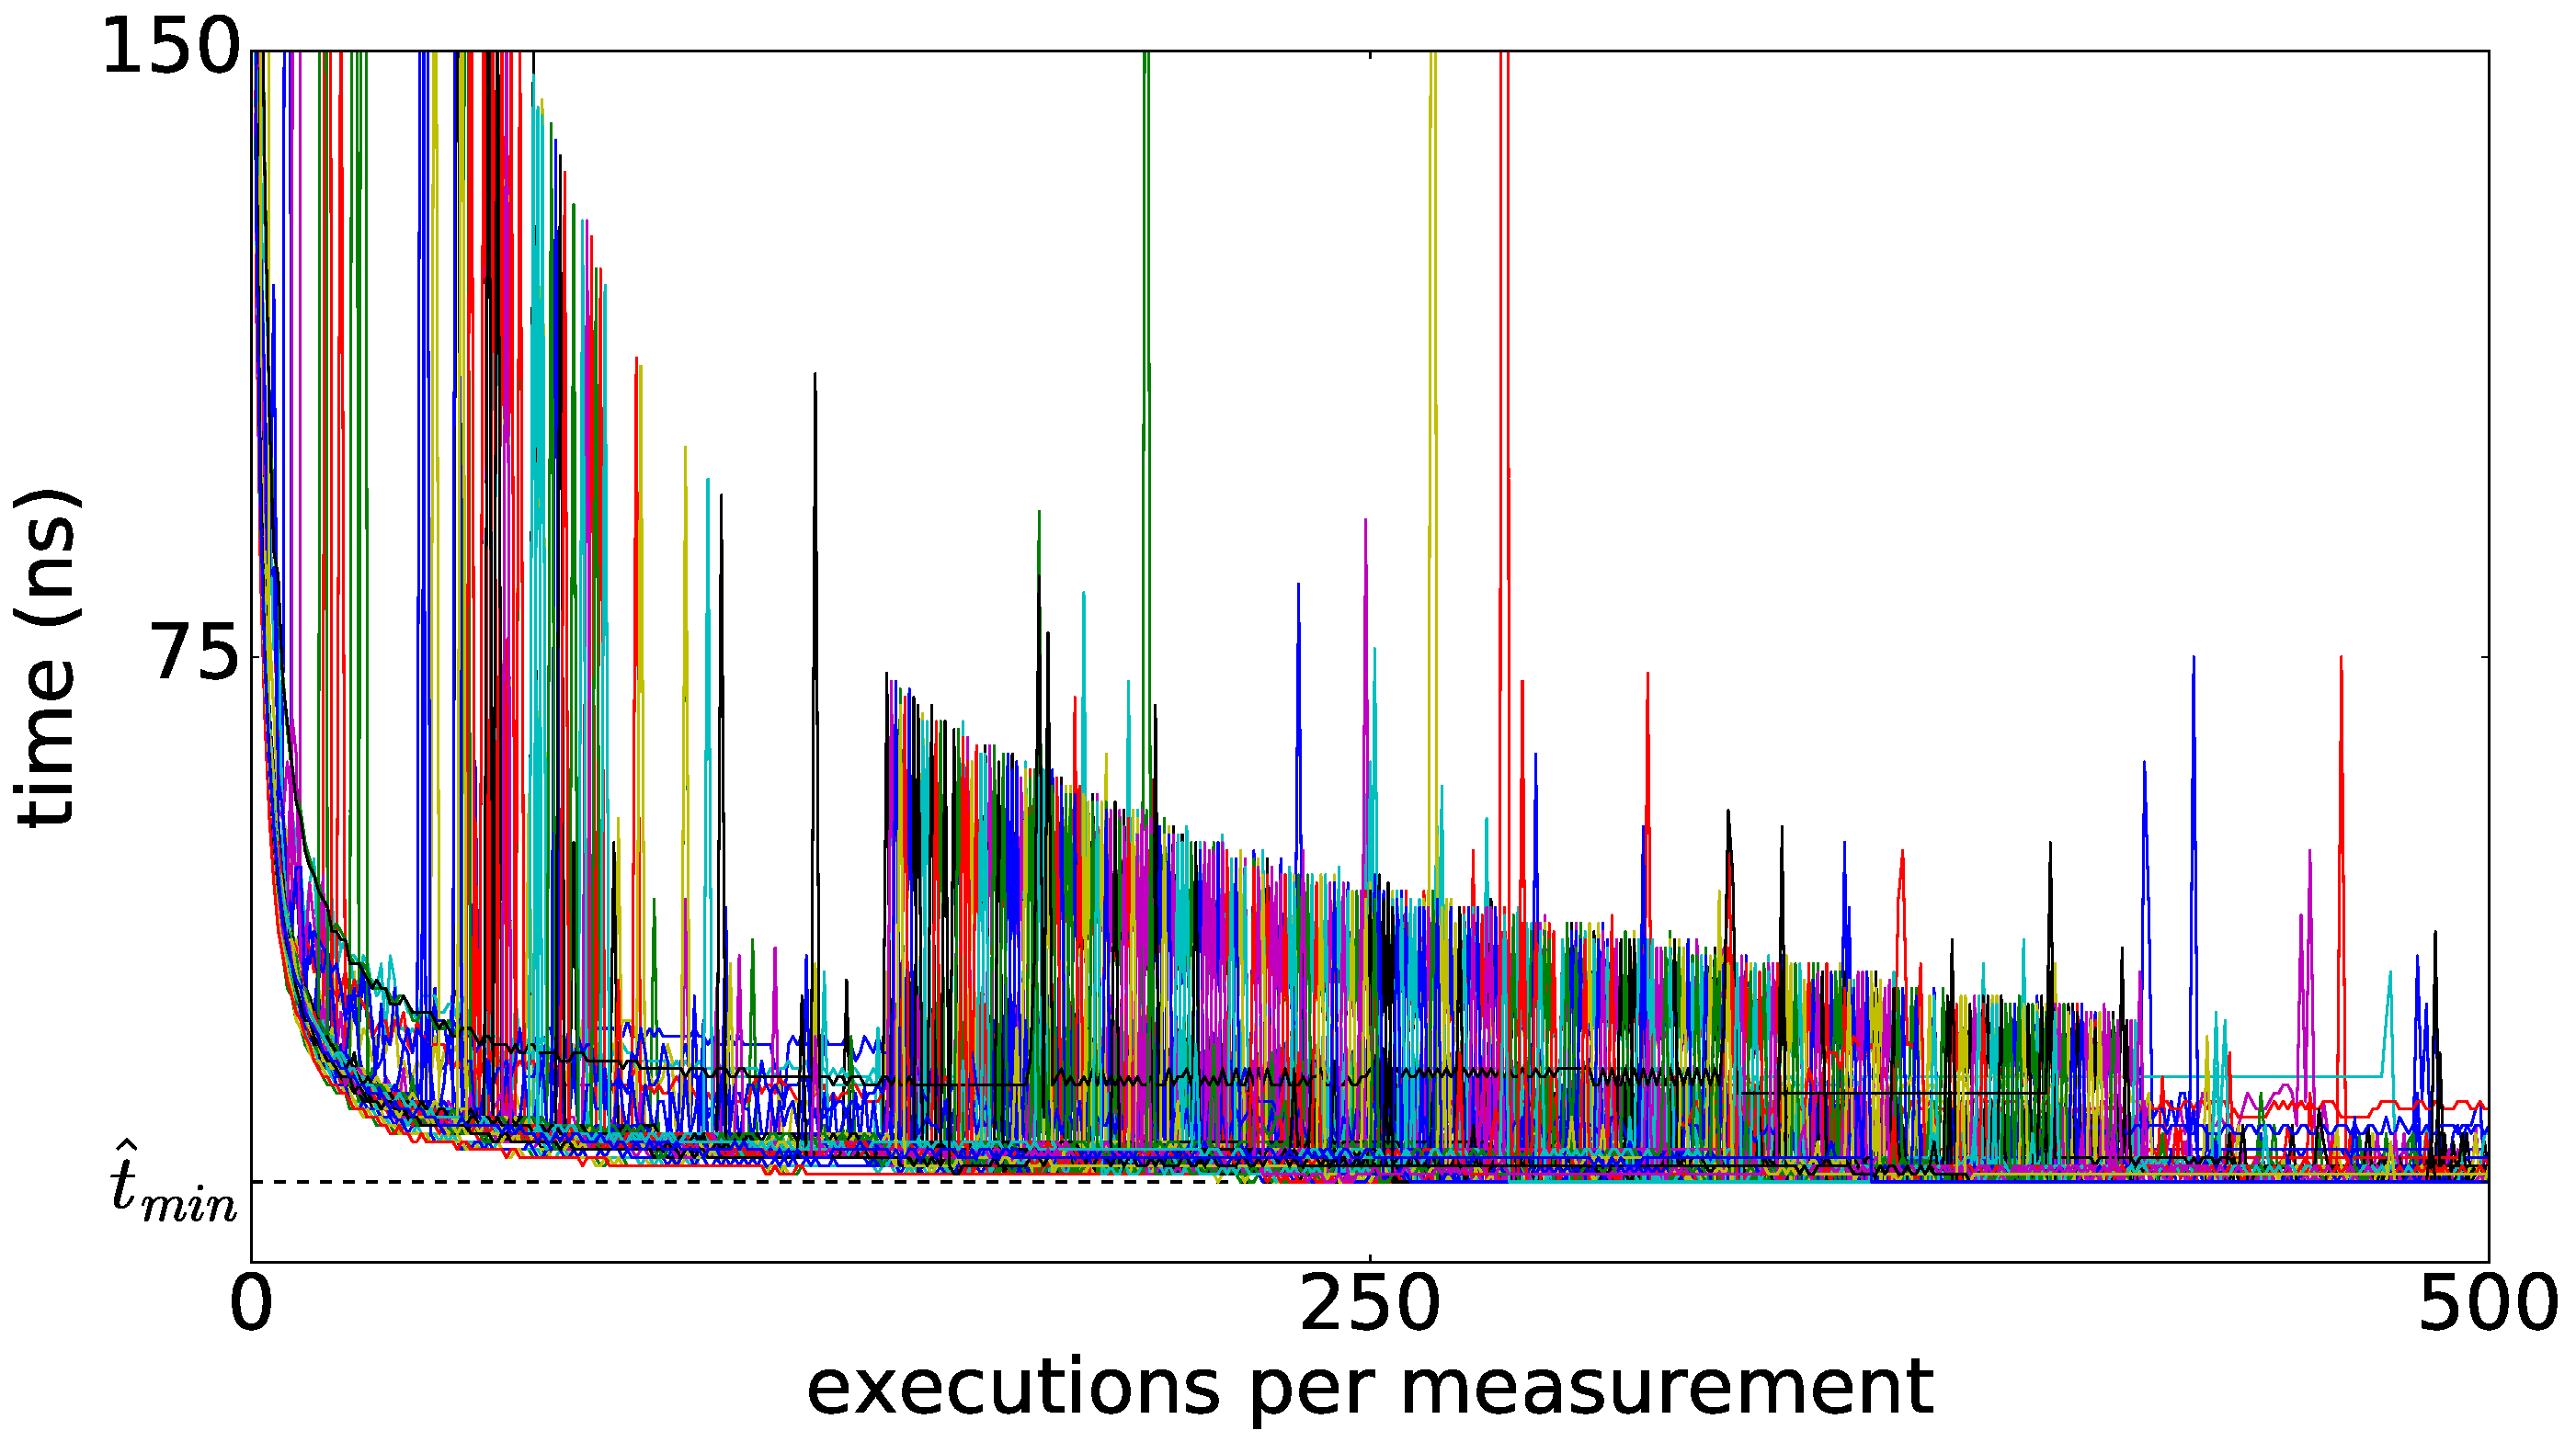
\includegraphics[width=\columnwidth]{figures/fig2/linear_scan_branchsum}
\caption{Each curve $i$ plots the coordinates
$\left(1, \frac{T^{\{i\}}_1}{1}\right), \dots,
\left(500, \frac{T^{\{i\}}_{500}}{500}\right)$
gained by executing Algorithm 1 with the same benchmark. Note the relative
smoothness and asymptotic behavior of the cross-curve minima.}
\label{fig:scaling}
\end{figure}

In our model, we choose to use the minimum estimator as opposed to the more commonly used
median or mean estimators. We made this choice because $\textrm{min}(\frac{T_1}{1}, \dots
\frac{T_{\tau_{\textrm{acc}}}}{\tau_{\textrm{acc}}})$ produces the closest estimate to
$t_{P_0}$ attainable from our sample. Let us justify this claim.

Consider the total error term for a given timing measurement $E_m = \frac{\left(\sum_{i}
X_Q^{(i)} \tau^{(i)} + \epsilon \right)_m}{n_m}$, such that $\frac{T_i}{n_i} = t_{P_0} +
E_i$. Using this notation, our justification for using the minimum to estimate $t_{P_0}$ can
be written:

\begin{align}
    \hat{t}_{P_0} &= \textrm{min}(\frac{T_1}{1}, \dots \frac{T_{\tau_{\textrm{acc}}}}{\tau_{\textrm{acc}}}) \\ \nonumber
                  &= \textrm{min}(t_{P_0} + E_1, \dots t_{P_0} + E_{\textrm{acc}}) \\ \nonumber
                  &= t_{P_0} + \textrm{min}(E_1, \dots E_{\textrm{acc}}) \\ \nonumber
\end{align}

\begin{figure}
\centering
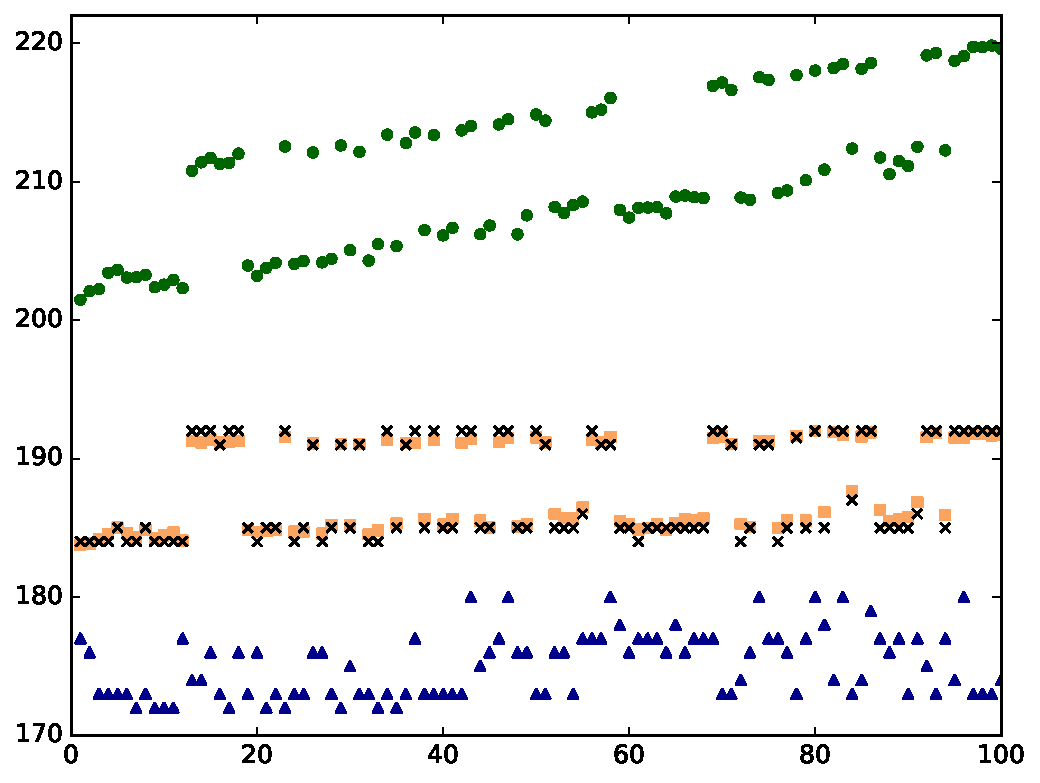
\includegraphics[width=\columnwidth]{figures/fig3/location_estimators_sumindex}
\caption{The behavior of different location parameters across multiple trials of
the \lstinline|sumindex| benchmark: mean (green filled circles), trimmed mean of
the 5th---95th percentiles (brown filled squares), median (black crosses), and
minimum (blue filled triangles).}
\label{fig:locationmeasures}
\end{figure}

The minimum thus inherently selects the estimate with the smallest error term.

This interpretation of the minimum is supported by the behavior of the timing estimate
curves plotted in Fig~\ref{fig:scaling}. These curves feature a relatively smooth lower
bound, to which the minimum converges after the region where timer accuracy has a
significant influence on the result.

Fig~\ref{fig:pdfsumindex} and Fig~\ref{fig:locationmeasures} provide further justification
for the minimum over other common estimators like the median, mean, or trimmed mean. Recall
from Section~\ref{sec:model} that the $E_i$ terms are sampled from a sum of scaled random
variables following nonidentical Poisson binomial distributions. As such, these terms often
exhibit multimodal behavior, as can be seen in the figures.

While estimators like the median and trimmed mean are known to be robust to
outliers~\cite{Maronna2006}, Fig~\ref{fig:locationmeasures} demonstrates that they still
capture bimodality of the distributions plotted in Fig~\ref{fig:pdfsumindex}. Thus, these
estimators are undesirable because our choice of $n$ could vary drastically between
different executions of Algorithm~\ref{alg:tuning}, depending on which of the estimator's
modes was captured in the sample.

By contrast, we see that the distribution of the minimum across all experimental trials is
unimodal, implying that the minimum is unaffected by the bimodally-distributed error terms.
\textbf{For our model, the minimum is a unimodal, robust estimator for the location
parameter of a given benchmark's timing distribution}.

\begin{figure}
\centering
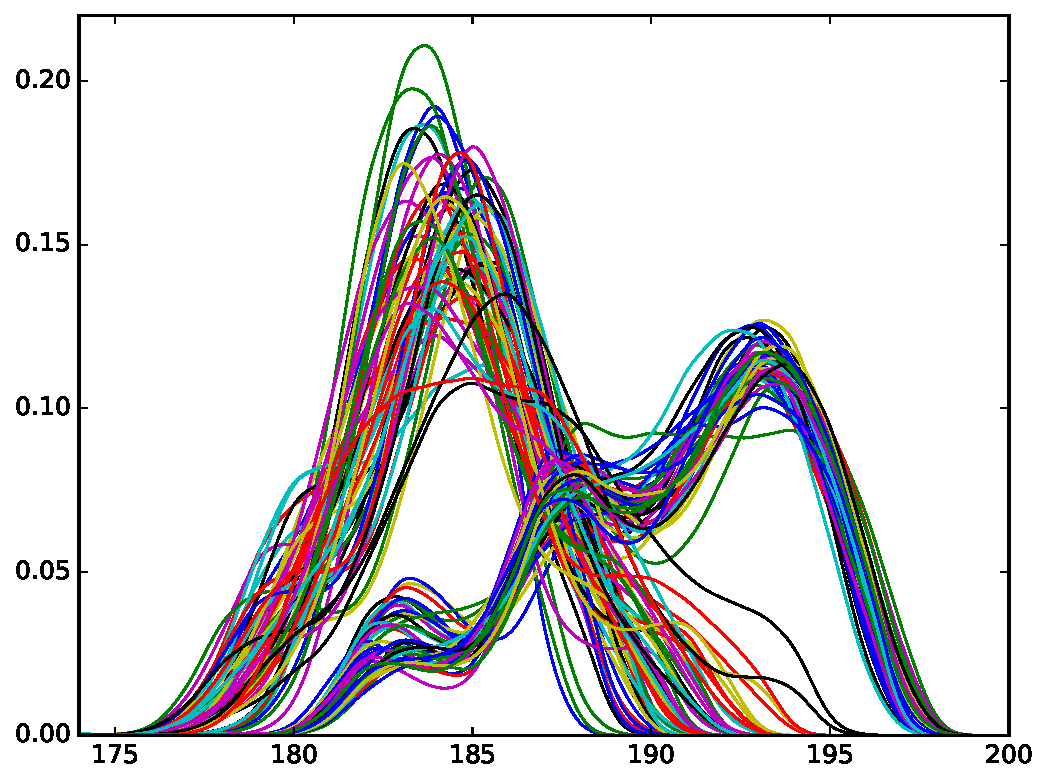
\includegraphics[width=\columnwidth]{figures/fig4/kde_pdf_sumindex}
\caption{Kernel density estimates (KDEs) of the probability density functions (pdfs)
across 100 trials of the \lstinline|sumindex| benchmark. Each individual line is
a KDE formed from a trial of 10,000 consecutively gathered timing measurements. Note that
the data forms two distinct clusters. A cursory investigation did not reveal any inter-trial
patterns or periodicity that might enable the naive prediction of any given trial's affinity
for one pdf or the other.}
\label{fig:pdfsumindex}
\end{figure}

\subsection{Justifying the $n$ range}

It might not be obvious why our heuristic does not test $n > j$, where
$j = \tau_{\textrm{acc}} / \tau_{\textrm{prec}}$. Recall
that $-\tau_{\textrm{acc}} \le \epsilon \le \tau_{\textrm{acc}}$. For a given value of $n$,
the timer error term in a timing estimate is $\frac{-\tau_{\textrm{acc}}}{n} \le
\frac{\epsilon}{n} \le \frac{\tau_{\textrm{acc}}}{n}$. Thus, when $n = j$:

\begin{equation}
\frac{-\tau_{\textrm{acc}}}{j} \le \frac{\epsilon}{j} \le \frac{\tau_{\textrm{acc}}}{j} \to -\tau_{\textrm{prec}} \le \frac{\epsilon}{\tau_{\textrm{acc}}} \le \tau_{\textrm{prec}}
\end{equation}

In other words, we do not test $n > j$ since the error at $n \ge j$ is constrained to timer
precision.

\subsection{The oracle function}
\label{sec:oracle}

Our heuristic takes as input an oracle function $\nu(t)$ that maps expected runtimes to an
optimal number of executions per measurement. While Algorithm 1 does not directly describe
$\nu(t)$, appropriate choices for this function should have the following properties (once
again setting $j = \tau_{\textrm{acc}} / \tau_{\textrm{prec}}$):

\begin{itemize}
    \item $\nu(t)$ has a discrete range $n \in \{1, \dots j\}$
    \item $\nu(t)$ is monotonically decreasing
    \item $\frac{d\nu}{dt}|_{t \approx \tau_{\textrm{prec}}} \approx 0$
    \item $\frac{d\nu}{dt}|_{t \approx \tau_{\textrm{acc}}} \approx 0$
    \item $\nu(\tau_{\textrm{prec}}) \approx j$
    \item $\nu(t \ge \tau_{\textrm{acc}}) \approx 1$
\end{itemize}

Some of the above properties require further motivation. First, $\nu(t)$ should be
monotonically decreasing because benchmarks with larger runtimes will require smaller $n$,
and vice versa. Second, $\nu(t)$ should be relatively flat for small $t$ because variations
in the error term between timing estimates can be large compared to the actual runtime of
fast benchmarks.

A useful realization of $\nu(t)$ is a special version of the generalized logistic function
that can be tuned to achieve the above properties. For our purposes, we can express this
function as

\begin{equation} \label{eq:14}
    Y(t) = \floor*{1 + \frac{\tau_{\textrm{acc}} - 1}{1 + e^{a * (t - b*\tau_{\textrm{acc}})}}}
\end{equation}

where reasonable values of $a$ and $b$ are approximately $0.005 < a < 0.02$ and $0.4 < b <
0.6$. In practice, we have found that more optimal results can be achieved by first
approximating $Y(t)$ with a lookup table, then modifying the lookup table based on empirical
observations. This was accomplished by examining many benchmarks with a variety of known
runtimes at different time scales, seeking for each runtime the smallest $n$ value at which
the minimum estimate appears to converge to a lower bound (e.g. around $n = 250$ for the
benchmark in Fig~\ref{fig:scaling}). Fig~\ref{fig:oracle} plots both Eq~\ref{eq:14} and an
empirically obtained lookup table as potential oracle functions.

\begin{figure}
\centering
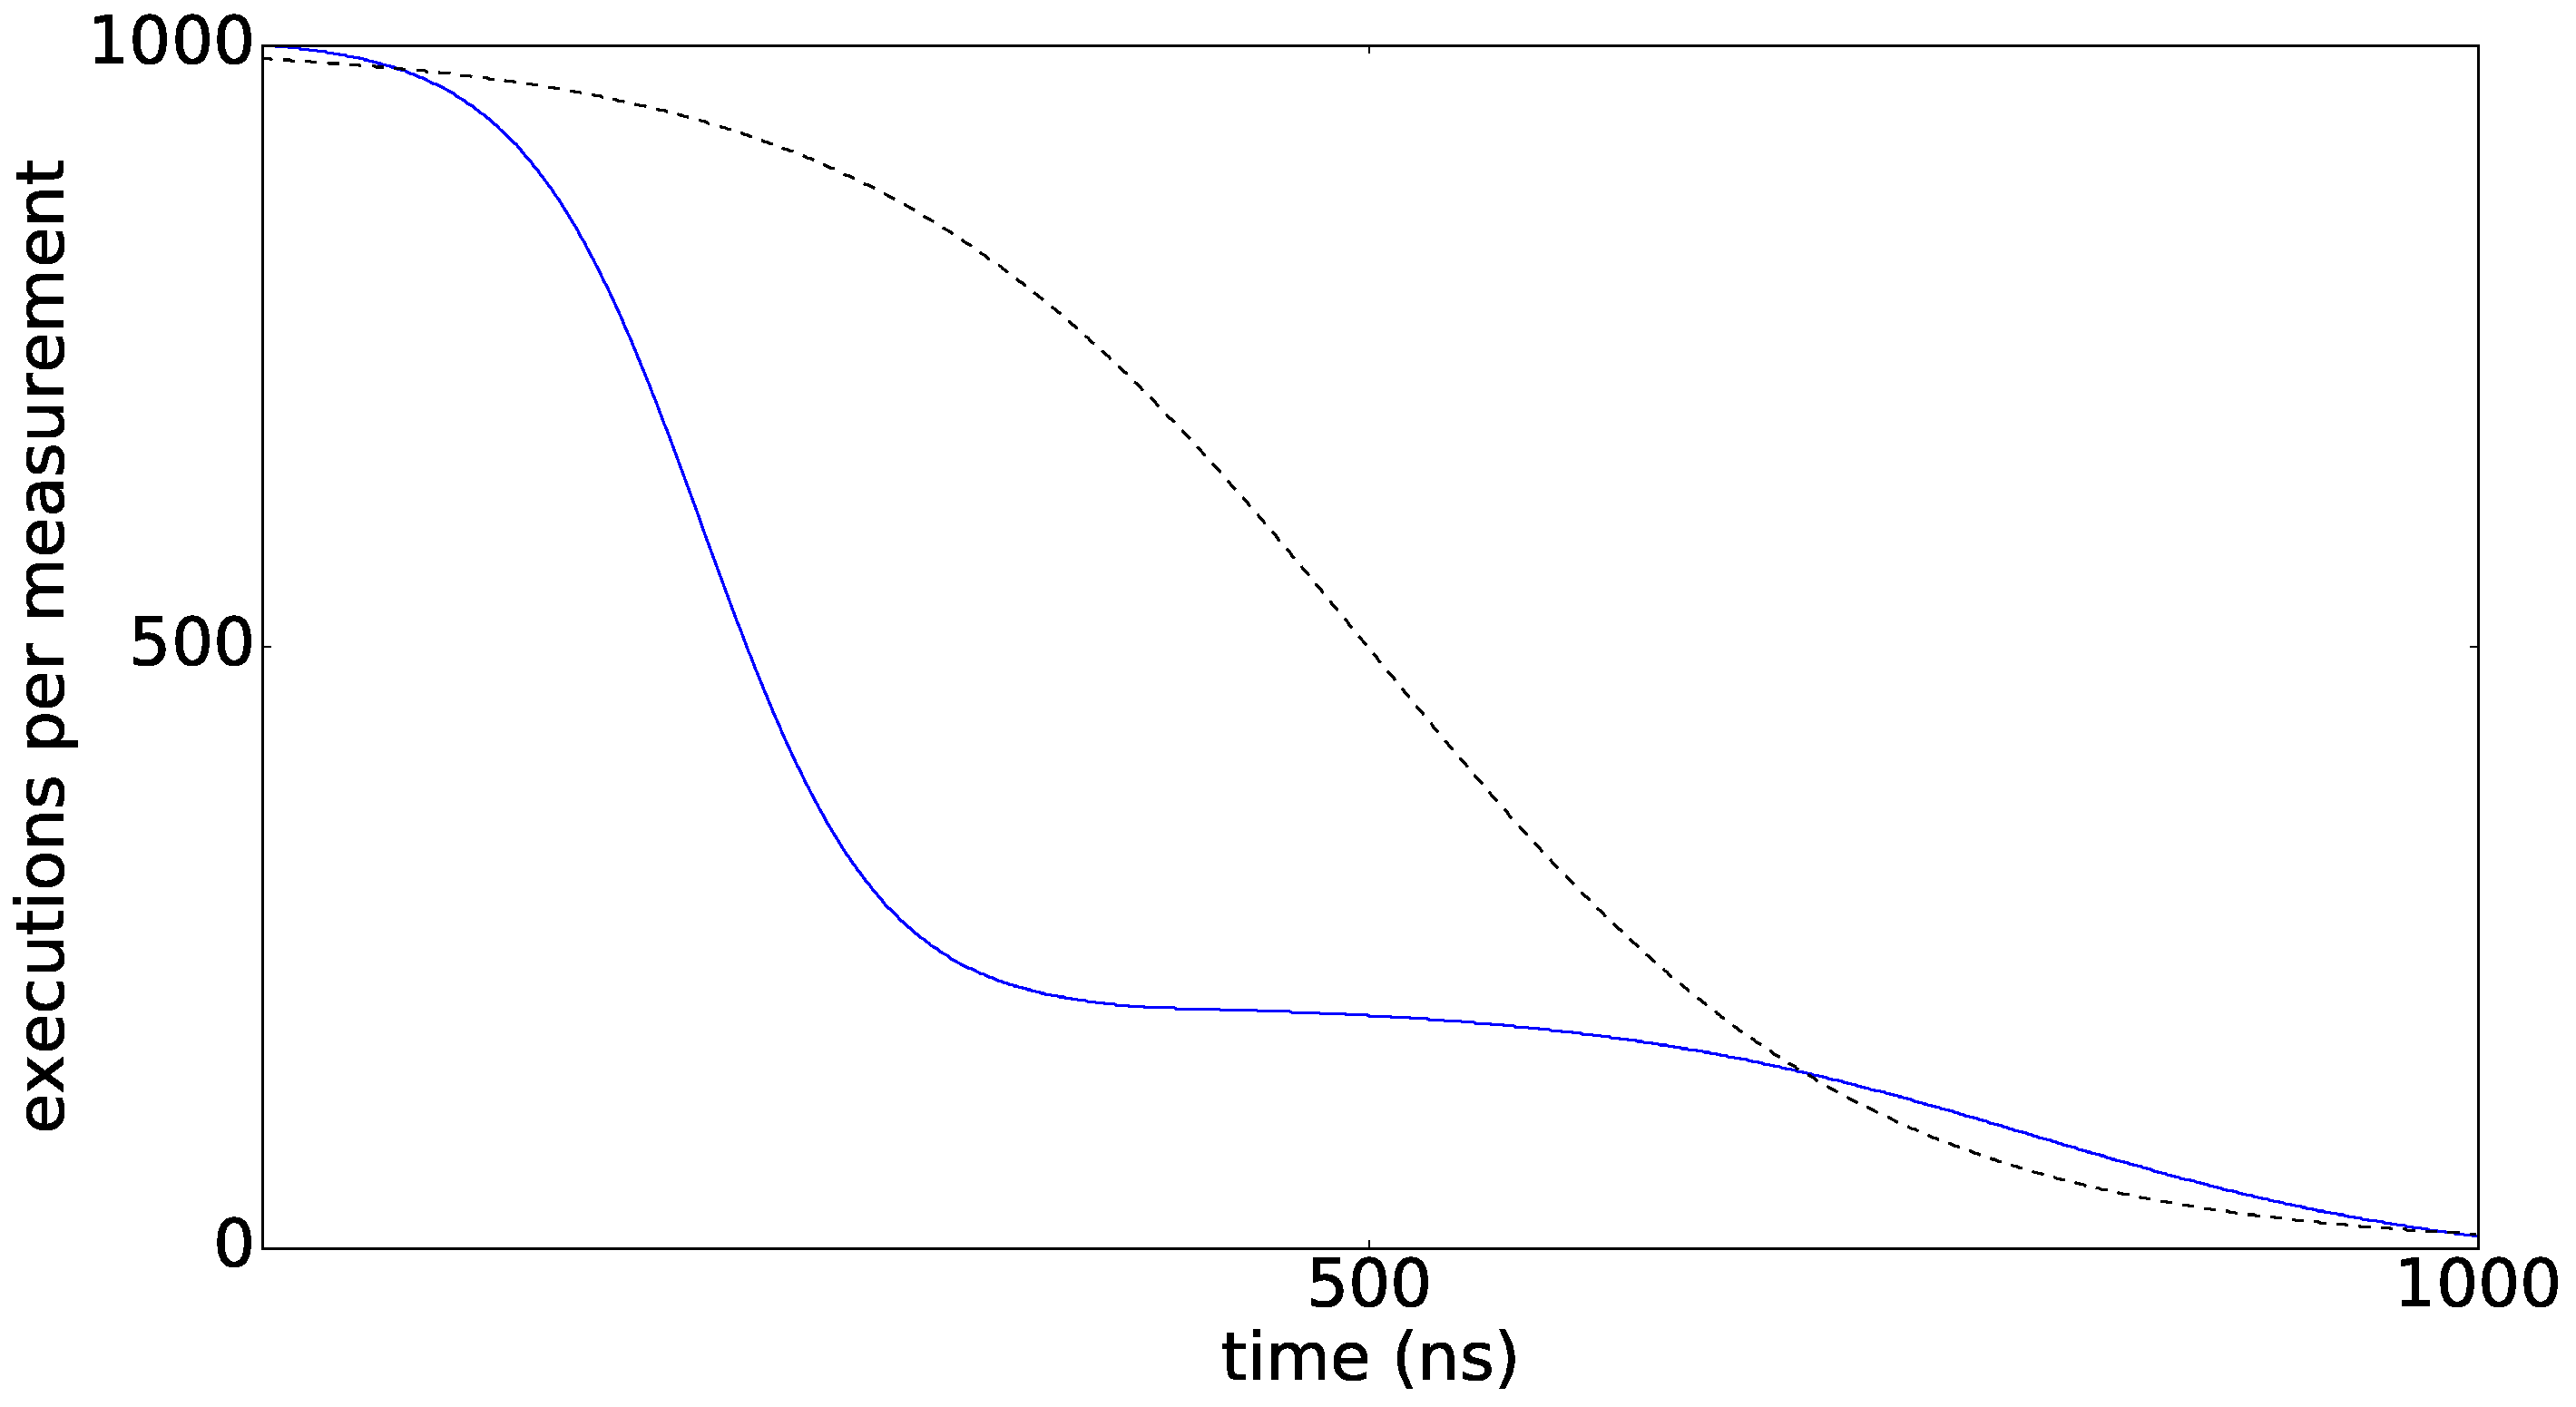
\includegraphics[width=\columnwidth]{figures/fig5/oracle}
\caption{Two possible curves for $\nu(t)$ at $\tau_{\textrm{acc}} \approx 1000 \textrm{ns}$.
The solid blue curve is an example of an empirically-tuned lookup table, while the dotted
black curve is $Y(t)$ from Eq~\ref{eq:14} with parameters $a = 0.009$ and $b = 0.5$.}
\label{fig:oracle}
\end{figure}

%%%%%%%%%%%%%%%%%%%%%%%%%%%%%%%%%%%%%%%%%%%%%%%%%%%%%%%%%%%%%%%%%%%%%%%%%%%%%%%%%%%%%%%%%%%%
\section{The difficulties of hypothesis testing and a potential way forward}
\label{sec:hypotesting}

A logical next step would be to use our model to compare the timing estimates of two
programs - or equivalently, two different versions of the same program - and provide to the
reader an algorithm for calculating some measure of the statistical significance of the
comparison, such as a confidence interval. Unfortunately, as mentioned in
Section~\ref{sec:toughstats}, many common statistical tests are inapplicable to our
model due to the non-i.i.d. (potentially even non-stationary) nature of benchmark timing
measurements.

For example, recall from Section~\ref{sec:model} that timing samples are drawn from a sum of
scaled random variables following nonidentical Poisson binomial distributions. Though this
technically constitutes a parameterized distribution, there are an overwhelming number of
parameters to take into account. While it is possible that some benchmarks' timing
distributions are feasibly derivable given extremely precise knowledge of the target program
and execution environment, it is safe to say that, in practice, the excessive number of
uncontrolled variables will generally render parametric hypothesis testing untenable.

Often, nonparametric tests are used when it is infeasible to analytically derive the
properties required by parametric tests. Consider the naive bootstrap, a popular
resampling-based nonparametric method for hypothesis testing. In this method, new samples
are randomly drawn from the original sample, in effect treating the original sample as an
estimate of the original population so that an estimate for the distribution of a test
statistic can be formed without prior knowledge of the original population's
distribution~\cite{Efron1992}. While the naive bootstrap can sometimes succeed in the
presence of non-identically distributed samples, it will generally fail when applied to
correlated samples, since the resample will fail to capture correlations in the original
sample~\cite{Mammen2012}. Luckily, statisticians have developed certain variants of these
methods which are designed to work for correlated data.

One of these variants is known as permutation testing, which can yield exact confidence
intervals as long as the two samples being compared were drawn from populations following
exchangeable distributions under the null hypothesis~\cite{Good2013}. The downside of
permutation testing is that it can be immensely computationally expensive for large sample
sizes, as it requires the test statistic to be calculated for many (if not all) permutations
of the two original samples.

Other resampling techniques, referred to as block resampling methods, preserve correlations
by randomly drawing whole blocks of consecutive measurements from the original sample,
rather than randomly drawing individual measurements. Well-known examples of block
resampling methods include the block bootstrap~\cite{Kunsch1989}, the stationary
bootstrap~\cite{Politis1994} and the block subsampling method~\cite{Politis1999}. The
computational feasibility and robustness of block resampling methods in the presence of
non-i.i.d., non-stationary, and even heteroskedastic behavior~\cite{Politis1999,Politis1997}
make them promising candidates for use in automated statistical performance regression
detection systems. The chief difficulty one faces when applying these methods is that they
feature a low tolerance for suboptimal choices of configuration parameters. For example,
these methods can fail to produce a uniform p-value distributions if the size of the
resampled block is not chosen properly~\cite{Shao2013}. Additionally, in order to prevent
degeneracy in the estimated distribution, one must apply a normalization coefficient to the
test statistic~\cite{Politis1999}. This coefficient is derived from the rate of convergence
of the statistic's variance with increasing sample size, which can depend on the original
population's underlying distribution.

In order to obviate the need for manual derivation of block sizes and normalization
coefficients, statisticians have proposed several automatable, data-dependent procedures for
selecting them~\cite{Politis2004,Bickel2008}. Furthermore, several augmentations have been
devised that can increase the statistical power of block resampling methods under suboptimal
or nontraditional choice of configuration parameters~\cite{Berg2010,Shao2013}. We believe
that an investigation of the applicability of these procedures, and block resampling methods
in general, could prove a fruitful avenue of future research for the study of statistical
regression detection.

%%%%%%%%%%%%%%%%%%%%%%%%%%%%%%%%%%%%%%%%%%%%%%%%%%%%%%%%%%%%%%%%%%%%%%%%%%%%%%%%%%%%%%%%%%%%
\section{Implementation in Julia}
\label{sec:implementation}

The experimental methodology in this paper is implemented in the \lstinline|BenchmarkTools|
Julia package\footnote{\url{https://github.com/JuliaCI/BenchmarkTools.jl}}. In addition to
the \lstinline|BaseBenchmarks|\footnote{\url{https://github.com/JuliaCI/BaseBenchmarks.jl}}
and \lstinline|Nanosoldier|\footnote{\url{https://github.com/JuliaCI/Nanosoldier.jl}}
packages, the \lstinline|BenchmarkTools| package implements the on-demand CI benchmarking
service used by core Julia developers to compare the performance of proposed language
changes with respect to over 1300 benchmarks. Since this CI benchmarking service began in
early 2016, it has caught and prevented the introduction of dozens of serious performance
regressions into Julia's standard library (defining a ``serious'' regression as a $30\%$ or
greater increase in a benchmark's minimum execution time).

The benchmarks referenced in this paper are Julia benchmarks written and executed using
\lstinline|BenchmarkTools|. A brief description of each benchmark is offered below:

\begin{itemize}
    \item The \lstinline|sumindex(a, inds)| benchmark sums over all \lstinline|a[i]| for all
    \lstinline|i| in \lstinline|inds|. This test stresses memory layout via element
    retrieval.
    \item The \lstinline|pushall!(a, b)| benchmark pushes elements from \lstinline|b| into
    \lstinline|a| one by one, additionally generating a random number at each iteration (the
    random number does not affect the output). This test stresses both random number
    generation and periodic reallocation that occurs as part of Julia's dynamic array
    resizing algorithm.
    \item The \lstinline|branchsum(n)| benchmark loops from \lstinline|1| to \lstinline|n|.
    If the loop variable is even, a counter is decremented. Otherwise, an inner loop is
    triggered which runs from \lstinline|1| to \lstinline|n|, in which another parity test
    is performed on the inner loop variable to determine whether to increment or decrement
    the counter. This test stresses periodically costly branching within loop iterations.
    \item The \lstinline|manyallocs(n)| allocates an array of \lstinline|n| elements, where
    each element is itself an array. The inner array length is determined by a random number
    from \lstinline|1| to \lstinline|n|, which is regenerated when each new array is
    constructed. However, the random number generator is reseeded before each generation so
    that the program is deterministic. This test stresses random number generation and
    the frequent allocation of arrays of differing length.
\end{itemize}

The mock benchmark suite referenced in this paper is hosted on GitHub at
\url{https://github.com/jiahao/paper-benchmark}.

%%%%%%%%%%%%%%%%%%%%%%%%%%%%%%%%%%%%%%%%%%%%%%%%%%%%%%%%%%%%%%%%%%%%%%%%%%%%%%%%%%%%%%%%%%%%
\section*{Conclusion}
\label{sec:conclusion}

In this article, we discussed how the complexities of modern hardware and software
environments can hinder the application of traditional statistics to performance testing. We
presented Julia benchmark runtime measurements exhibiting non-i.i.d behavior, violating the
statistical assumptions made by many existing benchmarking methodologies. We discuss a
benchmarking methodology that does rigorously consider the non-i.i.d. statistics of program
timing distributions \cite{Kalibera2013}, but find that their method requires an overbearing
amount of manual tuning for large and frequently revised benchmark suites, such as the Julia
language's standard library benchmark suite.

To aid in the design of future performance testing approaches, we presented a statistical
model for describing timing measurement distributions. Our model does not assume i.i.d.
statistics, and exhibits convergence properties which challenge the common rule of thumb
that simply running a benchmark for longer, or repeating its execution many times, can
render the effects of external variation negligible. Our model also shows that, unlike
arbitrary sources of variation, error due to timer inaccuracy can, in fact, be amortized
simply by running a benchmark long enough or executing it many times.

Leveraging the properties of our model, we devised an automatable, data-dependent heuristic
for selecting the minimum number of executions of a benchmark per measurement required to
defeat timer error. This heuristic is implemented by the \lstinline|BenchmarkTools| Julia
package, which is employed daily and on-demand as part Julia's continuous integration (CI)
pipeline to automatically evaluate the performance effects of proposed changes to Julia's
standard library, as well as to test the performance of user-authored Julia packages.

We additionally discussed the use of hypothesis testing for determining the statistical
significance of performance regressions. We argue that many parametric and nonparametric
hypothesis tests are unsuitable for this task, because their correctness has not been proven
in a non-i.i.d. regime. We propose that performance testing research would benefit from
further investigation of non-i.i.d., data-dependent hypothesis testing techniques such as
the block subsampling method.

Throughout the paper, we present real timing measurements taken from Julia benchmarks which
demonstrate the multimodal behavior predicted by our model and motivate the design of our
experimental methodology. Section~\ref{sec:implementation} describes our experimental mock
benchmark suite in detail, and provides a link to the suite's implementation.

%%%%%%%%%%%%%%%%%%%%%%%%%%%%%%%%%%%%%%%%%%%%%%%%%%%%%%%%%%%%%%%%%%%%%%%%%%%%%%%%%%%%%%%%%%%%
\section*{Acknowledgment}
\label{sec:acknowledgement}

We thank the many Julia developers, in particular Andreas Noack and Steven G.
Johnson of MIT, for many insightful discussions.

This research was supported in part by the U.S. Army Research Office under
contract W911NF-13-D-0001.

%%%%%%%%%%%%%%%%%%%%%%%%%%%%%%%%%%%%%%%%%%%%%%%%%%%%%%%%%%%%%%%%%%%%%%%%%%%%%%%%%%%%%%%%%%%%
\bibliography{biblio}
\bibliographystyle{IEEEtran}

% that's all folks
\end{document}
\grid
